\section{Razpoznavanje obrazov}
Razvoj algoritmov z namenom preseganja človeške zmogljivosti poteka tudi na področju razpoznavanja ljudi. V letih 2007--2015 so se vrstile številne študije primerjave med zmogljivostjo ljudi in takratnih najboljših algoritmov. Sprva so se raziskovalci osredotočali na enostavnejše probleme, kot so različni pogoji osvetlitve na slikah frontalnih obrazov. V \cite{otoole2007face} so tako primerjali natačnost algoritmov in ljudi na slikah FRGC izziva (angl Face Recognition Grand Challenge \cite{}). Za problem so izbrali ujemanje obrazov na parih slik, ki so jih z algoritmom po PCA (Principal components analysis) metodi razdelili na lahke in težke primere. Z različnimi eksperimentalnimi protokoli, ki so podrobneje opisani v \cite{otoole2007face}, so nato testirali $91$ ljudi ($45$ žensk in $46$ moških). Vsak merjenec je moral oceniti ujemanje para slik na lestvici 1--5. Tako so dobili ROC krivulje, ki so jih nato primerjali s krivuljami algoritmov. 

Njihovi rezultati so pokazali, da algoritmi prekašajo ljudi na enostavnih primerih, na težkih primerih pa so primerljivi z ljudmi. Z dodatno analizo, so nato pokazali, da razlike niso nastale, ker bi bili ljudje utrujeni. Eden izmed razlogov zakaj obstajajo razlike, bi lahko bil ta, da merjenci niso poznali obrazov na slikah \cite{otoole2007face}. Drugi razlog bi lahko bil, da so značilke na enostavnih slikah dobro primerljive \cite{otoole2007face}. Ta dodatna informacija, bi lahko bila bistvena za prekašanje ljudi. S tem so v \cite{otoole2007face} prišli do sklepa, da so po natančnosti algoritmi primerljivi s človeško zmogljivostjo. 

Zelo podobno primerjavo med algoritmi in ljudmi so naredili v \cite{otoole2008humans}, kjer so poleg FRGC uporabili še podatkovno bazo obrazov FRVT 2006. Tudi v tem delu so se osredotočili na primerjavo pod različnimi osvetlitvenimi pogoji in prišli do podobnih zaključkov, da so algoritmi uspešnejši od ljudi. Z združevanjem človeka in algoritmov z regresijo delnih najmanjših kvadratov so zmanjšali stopnjo napake iz \num{0.12} na \num{0.008} in tako izboljšali rezultate. Pri tem so prišli do sklepa, da obstajajo razlike v napakah, ki jih delajo ljudje in algoritmi \cite{otoole2008humans}.

Nadaljna testiranja na bolj zahtevnih podatkovnih bazah (GBU Phillips et al 11\cite{}) so pokazala, da je sklepanje o prekašanju ljudi napačno. Zato so se v \cite{otoole2012comparing} osredotočili na bolj sofisticirano primerjavo, saj so poleg nekontrolirane osvetlitve uporabili tudi dnevno spreminjanje videza ljudi, kot so frizura, obrazna mimika, uporaba očal in pokrival. Enako kot v prejšnjih delih, so tudi tu preverjali zmogljivost pri primerjavi parov slik. Slike so z najboljšim algoritmom za rapoznavanje obrazov razdelili na tri težavnostne stopnje. Ljudi so testirali na podoben način kot \cite{otoole2007face} in primerjali ROC krivulje ljudi in algoritmov.

Rezultati ROC krivulj iz \cite{otoole2012comparing} so prav tako pokazali, da algoritmi prekašajo ljudi na enostavnejših slikah in da so primerljivi na bolj težavnih. V nadaljnem testu so preverili še korelacijski koeficient med ljudmi in izbranim algoritmom in ugotovili, da so korelacije negativne in statistično pomembne. Prav tako so ugotovili, da med korelacijami obstaja raztros, kar nakazuje, da obstajajo razlike med ljudmi in algoritmi.  

S tovrstno primerjavo so se ukvarjali tudi v delu \cite{best2014unconstrained}. Tu so avtorji predstavili izsledke raziskovanja človeške natančnosti razpoznavanja obrazov na slikah in video posnetkih. Za eksperimente so uporabili LFW  in YTF podatkovno bazo. Podatke so zbrali s pomočjo Amazon Mechanical Turk spletne strani, kjer so merjenci morali določiti, če se na parih slik ali posnetkov pojavi ista oseba. V raziskavi je sodelovalo 307 oseb (\SI{27.4}{\%} iz ZDA in \SI{55.1}{\%} iz Indije). Rezultate so primerjali s \cite{kumar2011describable} in z algoritmom DeepFace \cite{taigman2014deepface}. 

\begin{figure}[!htbp]
	\centering
	\includegraphics[width=0.7\columnwidth]{bestrowden_1}
	\caption{Avtor človeka je \cite{humanicon} po licenci \url{https://creativecommons.org/licenses/by/3.0/legalcode}. Slike iz \cite{huang2007labeled}.}
\end{figure}


Za slike so \cite{best2014unconstrained} dobili \SI{98.3}{\%}  človeško natančnost, medtem ko so v \cite{kumar2011describable} za človeško natančnost določili \SI{99.2}{\%}. Algoritem DeepFace \cite{taigman2014deepface} je dosegel \SI{97.5}{\%} natančnost. Pri testiranju na video posnetkih je bila natančnost ljudi veliko slabša od algoritma (\proc{89.7} ZDA in \proc{88.6} Indija proti \proc{91.4}), vendar so ljudje prekašali algoritem s stališča TAR pri nizkih vrednostih FAR. Rezultati so povzeti v tabeli \ref{tab:best_1}.

\begin{table}[!htbp]
	\centering
	\centering
	\begin{tabular}{l S[table-format=1.2, round-mode=places, round-precision=2] S[table-format=1.2, round-mode=places, round-precision=2]}
		\toprule
		\textbf{Metoda \textbackslash{} FAR} & \thead{\proc{0.4}} & \thead{\proc{1.0}} \\
		\midrule
		Ljudje (ZDA) & 71.2 & 80.6 \\
		Ljudje (Indija) & 44.9 & 63.7 \\
		DeepFace \cite{taigman2014deepface} & 25.9 & 54.8 \\
		\bottomrule
	\end{tabular}
	\caption{}
	\label{tab:best_1}
\end{table}

Raziskovalci so v \cite{best2014unconstrained} ugotovili, da v podatkovnih bazah obstaja demografska pristranskost, saj večino ljudi izhaja iz zahodne Evrope. Prav tako so opazili vpliv znanih obrazov. Ljudje so se pri znanih obrazih odrezali bolje.

Z rezultati so v \cite{best2014unconstrained} prikazali, da obstajajo razlike v interpretaciji uspešnosti algoritmov ob uporabi različnih metrik. To lahko nakazuje na neprimeren način testiranja, ki vodi v napačno sklepanje. S tovrstno problematiko so se ukvarjali v \cite{phillips2014comparison}, kjer so predstavili novo ogrodje za primerjalno analizo. Relativno zmogljivost ljudi in algoritmov so karakterizirali z AUC statistiko in jo grafično predstavili na točkovnem grafu, kjer $x$ os predstavlja AUC za zmogljivost ljudi in $y$ os AUC za zmogljivost algoritmov. Točke pod diagonalo pomenijo, da so ljudje uspešnejši, točke nad diagonalo pa, da so uspešnejši algoritmi. Na tak način so ugotovili, da algoritmi prekašajo ljudi, ko obdelujemo frontalne obraze na slikah. V primeru video posnetkov pa so ljudje še vedno najboljši. To so razložili tako, da ljudje pri razpoznavanju dobro uporabljamo tudi druge značilnosti na sliki, kot so deli telesa, medtem ko algoritmi tega ne zmorejo.

\begin{figure}[!htbp]
	\centering
	\includegraphics[width=0.7\columnwidth]{phillips2014comparison}
	\caption{}
\end{figure}

V \cite{phillips2015human} so ravno tako poskušali izboljšati protokole primerjanja. Predstavili so nov način pridobivanja človeške zmogljivosti (zlivanje), s katerim dobimo višje ocene. Po standardnem načinu (združevanje) vsak merjenec oceni ujemanje parov slik ali posnetkov na skali 1--5. Iz zbranih podatkov nato izračunamo ROC krivuljo. Po novem načinu pa pred izračunom ROC krivulje zbrane ocene še povprečimo. Primerjavo med načinoma za težje primere slik lahko vidimo v tabeli \ref{tab:phillips_pasc}. Podatki so zbrani iz \cite{phillips2015human}. Z novim načinom dobimo višje ocene človeške zmogljivosti tako za slike kot video posnetke. 


\begin{figure}[!htbp]
	\centering
	\includegraphics[width=0.7\columnwidth]{phillips2015human}
	\caption{Avtor človeka je \cite{humanicon} po licenci \url{https://creativecommons.org/licenses/by/3.0/legalcode}. Slike iz \cite{huang2007labeled}.}
\end{figure}


\begin{table}[!htbp]
	\centering
	\begin{tabular}{l S[table-format=1.3, round-mode=places, round-precision=2] S[table-format=1.3, round-mode=places, round-precision=2]}
		\toprule
		\textbf{Metoda} & \thead{AUC (slike)} & \thead{AUC (posnetki)} \\
		\midrule
		Združevanje & 0.859 & 0.943 \\
		Zlivanje & 0.990 & 0.998 \\
		\bottomrule
	\end{tabular}
	\caption{}
	\label{tab:phillips_pasc}
\end{table}

Z novo metodo računanja človeške zmogljivosti so v \cite{phillips2015human} pokazali, da v težkih primerih človeško zmogljivost doseže le en algoritem. V ekstremno težkih primerih pa rezultati kažejo na to, da je zmogljivost ljudi boljša od naključja, zmogljivost algoritmov pa ne.

Pomembna odkritja na področju nestandardne primerjalne analize so dobili tudi \cite{richardwebster2018visual}. V razpoznavanje obrazov so uvedli vizualno psihofiziko, kot je bila predstavljena že v poglavju \ref{sec:psihofizika}. Delovanje algoritmov so predstavili s krivuljo odziva v odvisnosti od izbrane popačitve slike. Po nedavnih rezultatih na podatkovnih bazah bi verjeli, da se najbolje obnesejo algoritmi, ki temeljijo na nevronskih mrežah. Presnetljivo pa so izbrani stresni testi pokazali, da eden izmed slabših algoritmov OpenBR \cite{a}, ki temelji na ročno izdelanih značilkah LBP \cite{a} in SIFT \cite{a} prekaša DNN algoritma FaceNet \cite{a} in OpenFace \cite{a}. Kot so poudarili v \cite{richardwebster2018visual}, rezultati nakazujejo na to, da ni vedno mogoče določiti robustne značilke z učenjem na veliki množici podatkov.


\begin{figure}[!htbp]
	\centering
	\includegraphics[width=0.7\columnwidth]{richardwebster_2}
	\caption{Slike iz \cite{jain2010fddb}.}
\end{figure}


V \cite{richardwebster2018visual} so predstavili tudi izsledke pri primerjavi z ljudmi. Merjencem so najprej prikazali sliko za \SI{50}{\ms} in nato barvni šum za \SI{500}{\ms}. Zatem so dobili $3$ slike izmed katerih so morali izbrati najbolj podobno sliko prvi. Ugotovili so, da je delovanje algoritmov in ljudi konsistentno le pri Gaussovem glajenju in zmanjševanju kontrasta. 

Vsa omenjena dela na področju razpoznavanja obrazov lepo nakazujejo na dve temeljni problematiki, ki se pojavljata pri primerjanju zmogljivosti ljudi in algoritmov. Prva izhaja iz same podatkovne baze. S podatkovnimi bazami zelo težko zajamemo kompleksnost... Kot sta pokazala že \cite{a} in \cite{b} so baze pristranske... 

Druga problematika temelji na načinu primerjanja človeške in algoritmične zmogljivosti. Kot sta pokazala \cite{best2014unconstrained} in \cite{phillips2014comparison}, metrike, ki so splošno uporabljene na področju razpoznavanja obrazov, lahko vodijo v napačno interpretacijo rezultatov... 
